%----------------------------------------------------------------------------------------
%	PACKAGES AND OTHER DOCUMENT CONFIGURATIONS
%----------------------------------------------------------------------------------------

\documentclass[sigconf]{acmart}

\usepackage[english]{babel}

\settopmatter{printacmref=false}
\renewcommand\footnotetextcopyrightpermission[1]{}
\pagestyle{plain}

\usepackage{titlesec} % Allows customization of titles
\titleformat{\section}[block]{\large\scshape\leftalign}{\thesection.}{1em}{}
\titleformat{\subsection}[block]{\large}{\thesubsection.}{1em}{}

\usepackage{hyperref}

%----------------------------------------------------------------------------------------
%	TITLE & AUTHORS SECTION
%----------------------------------------------------------------------------------------

\begin{document}

\title{Recognizing emotions with technology and starting discussions}
\subtitle{Research in Emerging Technologies 2017-2018, final paper}
\date{January 2018}

\author{Randall Theuns}
\affiliation{%
    \institution{Amsterdam University of Applied Sciences}
    \department{Software Engineering}
    \streetaddress{Wibautstraat 2-4}
    \city{Amsterdam}
    \postcode{1091GM}
    \country{The Netherlands}
}
\email{randall.theuns@hva.nl}

\author{Max Beije}
\affiliation{%
    \institution{Amsterdam University of Applied Sciences}
    \department{Business IT \& Management}
    \streetaddress{Wibautstraat 2-4}
    \city{Amsterdam}
    \postcode{1091GM}
    \country{The Netherlands}
}
\email{max.beije@hva.nl}

\author{Frank Portengen}
\affiliation{%
    \institution{Amsterdam University of Applied Sciences}
    \department{Business IT \& Management}
    \streetaddress{Wibautstraat 2-4}
    \city{Amsterdam}
    \postcode{1091GM}
    \country{The Netherlands}
}
\email{frank.portengen@hva.nl}

\begin{abstract}
\noindent
According to Waag Society and the Research Group Crossmedia, recent studies have shown that
young adults are hard to reach when it comes down to (cultural) heritage.
Waag Society is researching how cultural heritage institutions can connect to these groups and 
how heritage objects can be relevant to (young) people.
Both parties believe that a better understanding of the emotions people have,
is very important to learn more about the way people value cultural heritage.
Therefore, Waag Society and the Research Group Crossmedia asked students of the HvA to
design an interactive tool that captures young adults’ emotions and enables them to discuss
these emotions with their peers when looking at (cultural) heritage.
\end{abstract}

\maketitle

%----------------------------------------------------------------------------------------
%	ARTICLE CONTENTS
%----------------------------------------------------------------------------------------

\section{Keywords}
Facial recognition, prototype, emotions, heritage, discussion, expressions

%------------------------------------------------

\section{Introduction}
During the minor 'Research in Emerging Technologies', we've chosen the project 'Emotions in Heritage' that
is commissioned by the Research Group Crossmedia (HvA) and the Waag Society. The Waag Society explores
emerging technologies not only related to the internet, but also related to biotechnology and cognitive sciences.
Art and culture often plays a central role in our research as well.

Our project involves systematically collecting the different emotions people experience when they perceive
(cultural) heritage, and use this information to spark meaningful conversations between different parties
by visualizing the different emotions. Cultural heritage could, for example, mean a painting, a building, or
even a tradition. Earlier research regarding emotion recognition has already been conducted. However, these
researches were mostly conducted from a psychological point of view; what emotions are being expressed
and why do young adults express a specific emotion? As such, models to define the emotions already exist.
Currently, there is a lack of instrumentation to capture these emotions and allow young adults to openly discuss
their emotions regarding heritage.

There are many options available to recognize emotions. For example, facial expression recognition, voice
recognition, text recognition, and wireless signals. Initially, we did research regarding these different
methods. We found a paper \cite{den2005facereader} which contained the various recognition methods and also included
the accuracy with which they were able to recognize emotions. Using these measurements, we made the choice to
limit how our project will recognize emotions to the method with the highest accuracy. The result of this
research concluded that facial expression recognition had the highest accuracy at an average of ~94.48\%
\begin{figure}[h]
    \centering
    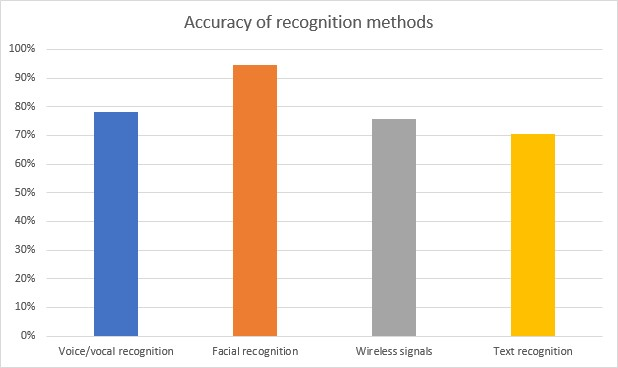
\includegraphics[width=0.45\textwidth, scale=1]{emotion_recognition_accuracy.jpg}
    \caption{Accuracy of recognition methods}
\end{figure}

Besides accuracy, two more restraints are defined:
\begin{enumerate}
    \item{If at all possible, all code and libraries used must be open source.}
    \item{The prototype has to display the predicted emotions in an interactive way.}
\end{enumerate}
Due to these requirements, and our choice to use facial expression recognition, the main research question
of this paper is: \emph{Does the visualization of emotions of young people (aged 16-26) by facial expression
recognition software, lead to discussion regarding the displayed content?}

By working towards answering this question, we are developing a prototype that collects the relevant information
that is required for the goal of the project: starting a meaningful conversation between young adults, regarding
a specific subject. Furthermore, if the prototype proves to be useful and provides valid data, it might be used in subsequent
research as a tool for collecting data.

%------------------------------------------------

\section{Related work}
Our project, as defined by the Waag Society, is already based on two previous research projects. The first
project explores a method to sympathize with other people's emotions around heritage objects. Young people,
teachers, and heritage professionals each map their emotions around a certain heritage topic and use that
mapping as a starting point for discussion \cite{emotionnetworking2017}. The goal of this research is very
similar to our own, however the means to reach that goal differ, in that our research aims to use technology
to read the emotions of the participants, as opposed to mapping them themselves.

The second project examines how participation, narratives, digital media, and atmosphere affect museum 
visitors when visiting an exhibition and how exhibition makers can influence these visitor experiences. 
One of the research questions is how people are emotionally affected when encountering one of 
these means \cite{}. Just like the first project, our research differs due to our focus on the technological
aspect of detecting emotions.

Besides the above two project which were already defined at the start of the project, we've also found research
conducted towards facial expression recognition \cite{den2005facereader}. This research focuses solely on
detecting emotions using a camera. We also had the opportunity to try out the software created during this
research. Unlike this research, our research also seeks to visualize these predicted emotions in a meaningful
way in order to spark a discussion.

Lastly, we found a series of articles that aim to create open source facial expression recognition software
\cite{gent2016landmarks}. All of the chosen libraries and datasets were open source or easily available.
We have chosen these articles as the basis for our own prototype.

%------------------------------------------------

\section{Methods}
To be added

%------------------------------------------------

\section{Results}
To be added

%------------------------------------------------

\section{Discussion}
To be added

%------------------------------------------------

\section{Acknowledgment}
This research was supported by the Amsterdam University of Applied Sciences, the Waag Society research
institute, and Research Group Crossmedia. We thank Bernadette Schrandt for all the assistance
with the research, including guidance and feedback. We thank Lodewijk Loos and Douwe-Sjoerd Boschman 
from Waag Society for the assistance during the creation of the prototype. We thank Wouter Meys for setting
up the minor and assisting with the research. Lastly, we would like to thank all the participants who helped
us test our final prototype.

%----------------------------------------------------------------------------------------
%	REFERENCE LIST
%----------------------------------------------------------------------------------------

\bibliographystyle{ACM-Reference-Format}
\bibliography{paper}

%----------------------------------------------------------------------------------------

\end{document}
